\documentclass{beamer}
\usepackage{etoolbox}\newtoggle{printable}\togglefalse{printable}
\usetheme{default}
\usecolortheme{beaver}
\usepackage{listings}
\usepackage{algpseudocode}
\pdfmapfile{+sansmathaccent.map}
\graphicspath{ {Images/} }

\title{Comp310 Demake Proposal}
\author{Alastair Rayner}
\date{\today}

\begin{document}

\maketitle


\begin{frame}{About the DeMake}
	  For this Demake project i will be creating Overcooked for the NES. \pause
	  
	  The game will be called Undercooked.\pause
	  
	 This presentation will cover the Concept, Mechanics and Technical Feasibility of the game. \pause
\end{frame}

\begin{frame}{About Overcooked}
    \textbf{Overcooked Examples}
    \center{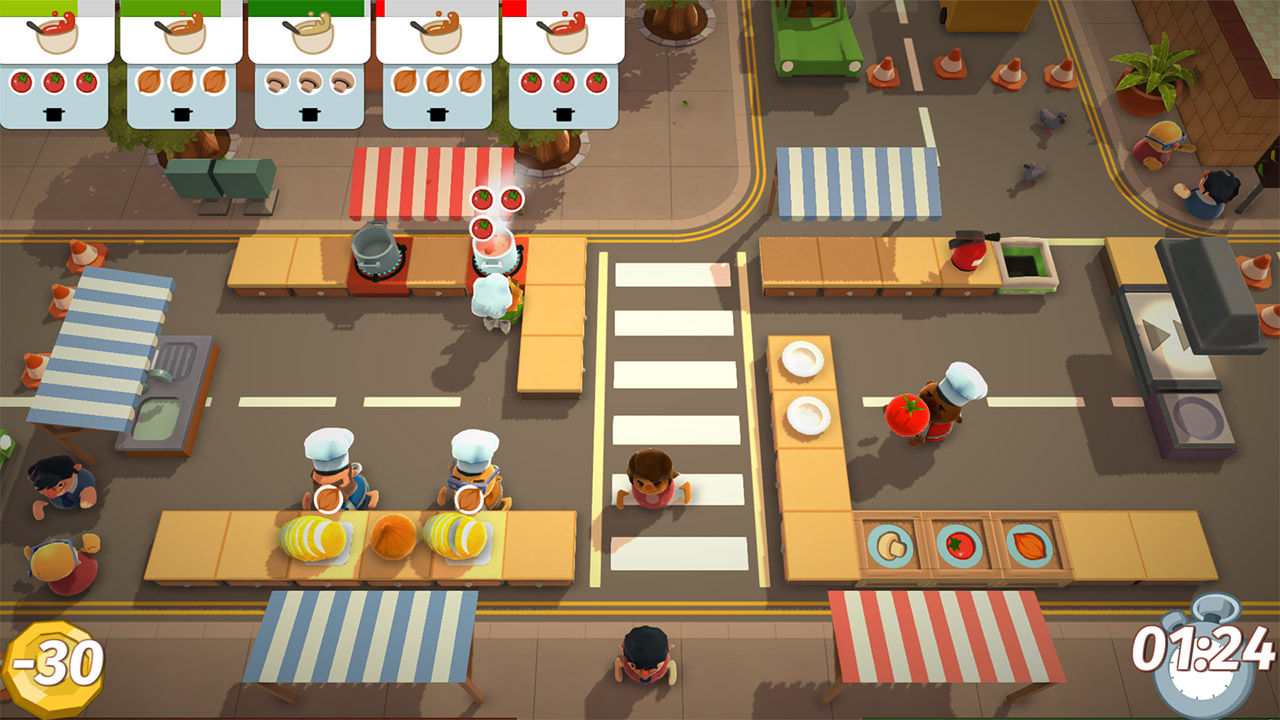
\includegraphics[width=10cm]{Overcooked1}}
    \textit{Image From:} www.psnation.com
\end{frame}

\begin{frame}{About Overcooked}
    \textbf{Overcooked Examples}
    \center{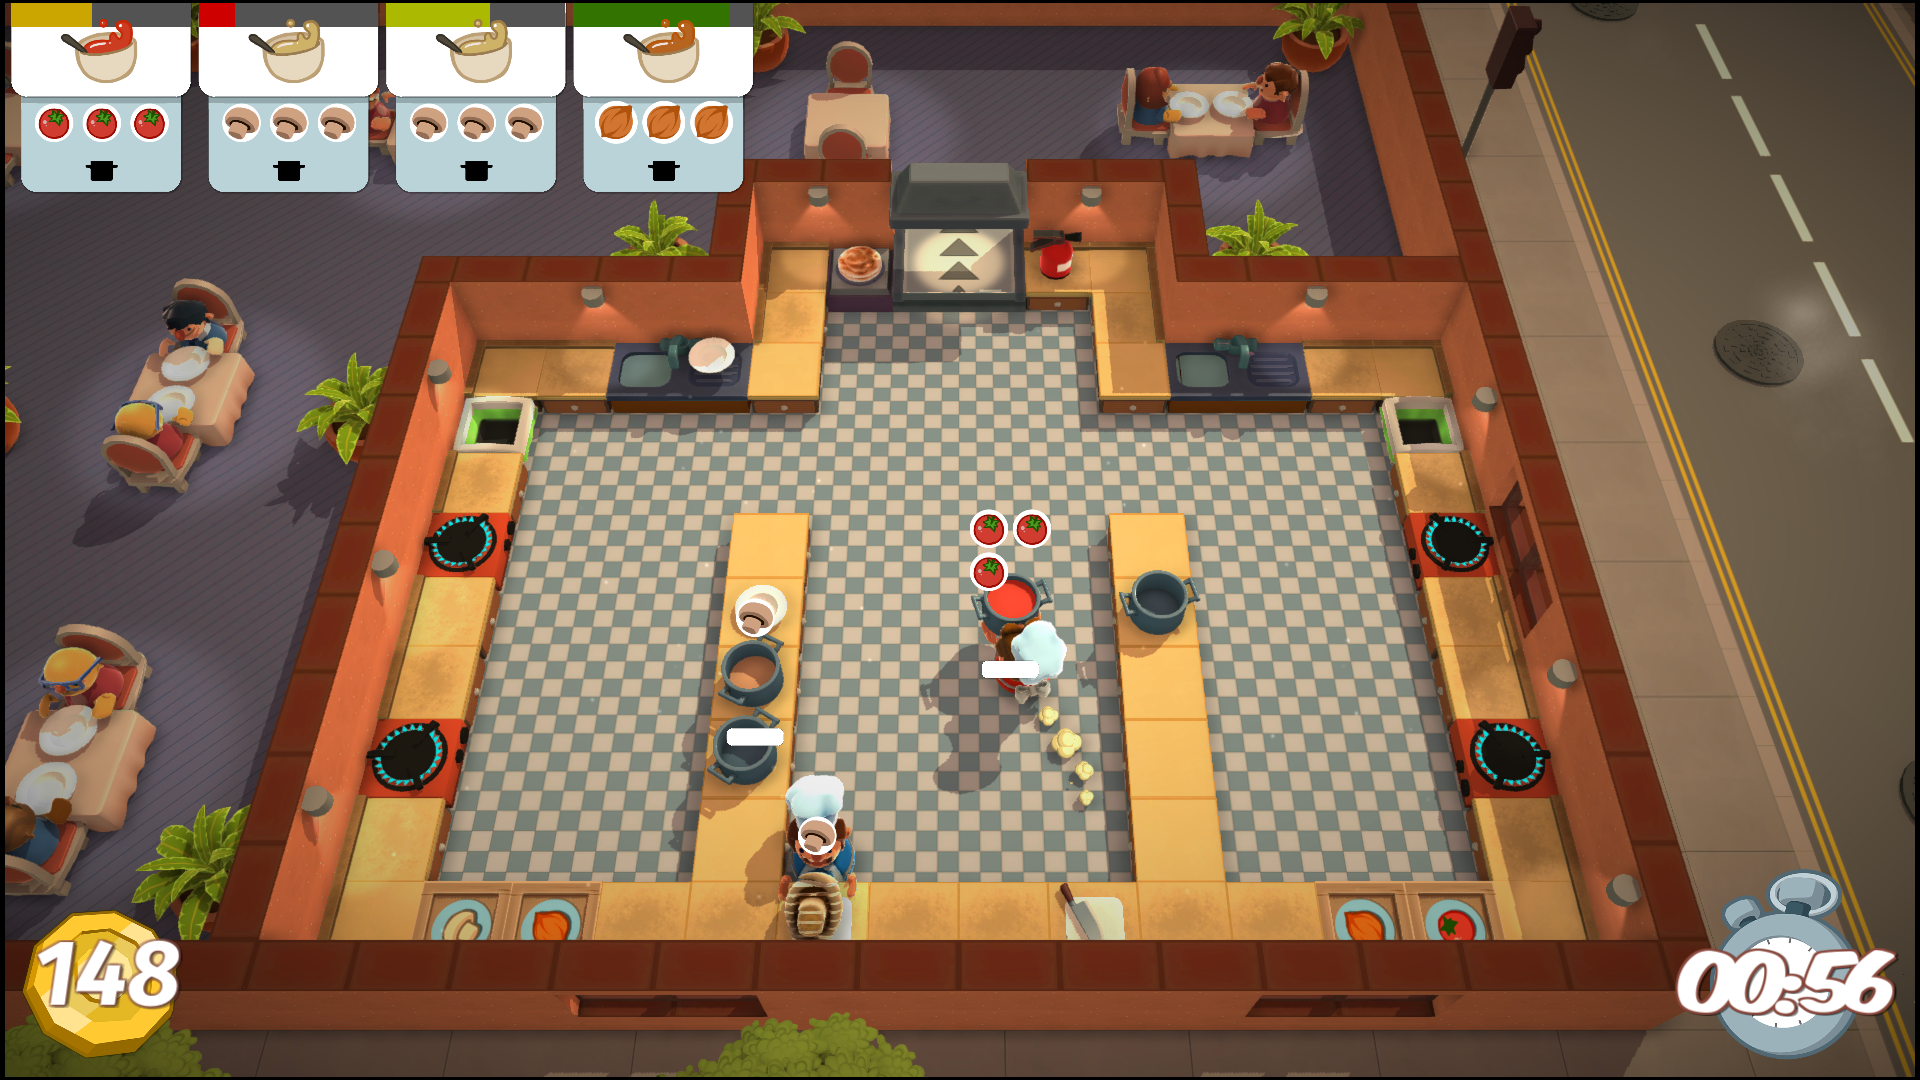
\includegraphics[width=10cm]{Overcooked2}}
    \textit{Image From:} images.nintendolife.com
\end{frame}

\begin{frame}{About Overcooked}
    \textbf{Overcooked Examples}
    \center{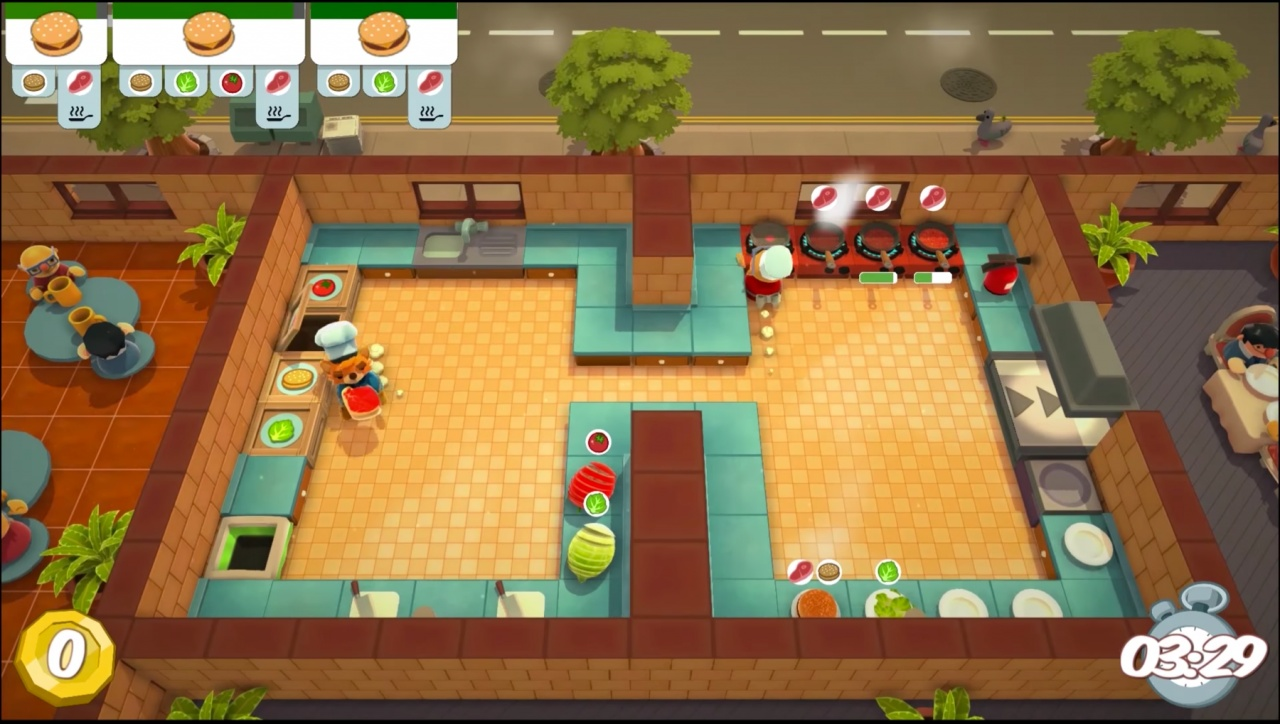
\includegraphics[width=10cm]{Overcooked3}}
   \textit{Image From:} images.nintendolife.com
\end{frame}

\begin{frame}{Concept}		
	\textbf{Game Concept} \pause
		\begin{itemize}
			\item The concept of my demake is a 2D top down cooking game, where the player has to create food as ordered before the time runs out. \pause
			\item The game can be co-op as well as single player. \pause
			\item However co-op will be a stretch goal. \pause
			\item The players score will increase with every correctly cooked item served. \pause
			
		\end{itemize}
\end{frame}

\begin{frame}{Key Mechanic}		
	\textbf{Core Mechanics} \pause
		\begin{itemize}
			\item Moving items around a kitchen and doing it as efficiently as possible.  \pause
			\item The stretch goals will be to implement co-op and have different levels \pause
			\item Also have disasters that happen, such as fire that spawns when food is cooked for too long. \pause
			

		\end{itemize}
\end{frame}

\begin{frame}{Technical Feasibility}		
	\textbf{Technical Feasibility} \pause
	
		\begin{itemize}
			\item This type of game is fairly simple, as there is no scrolling backgrounds, and not lots of enemies to render, only the player and the objects that the player can interact with. \pause
			\item The game will have a detailed player sprite, consisting of 4 8x8 sprites, and the tiles will be 8x8 sprites.  \pause
			\item The game will have pre-designed levels that the player can walk around in, and interact with certain usable cells, i.e. cooker, chopping board ect. \pause
			
		\end{itemize}
\end{frame}

\begin{frame}{Technical Feasibility}
    \textbf{The Legend of Zelda}
    \center{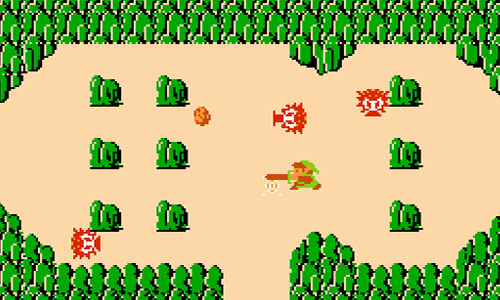
\includegraphics[width=10cm]{Zelda1}}
    \textit{Image From:} www.emuparadise.me
\end{frame}


\end{document}
